% Options for packages loaded elsewhere
\PassOptionsToPackage{unicode}{hyperref}
\PassOptionsToPackage{hyphens}{url}
%
\documentclass[
]{article}
\usepackage{amsmath,amssymb}
\usepackage{lmodern}
\usepackage{iftex}
\usepackage{fancyhdr}

\usepackage{titlesec}
\ifPDFTeX
  \usepackage[T1]{fontenc}
  \usepackage[utf8]{inputenc}
  \usepackage{textcomp} % provide euro and other symbols
\else % if luatex or xetex
  \usepackage{unicode-math}
  \defaultfontfeatures{Scale=MatchLowercase}
  \defaultfontfeatures[\rmfamily]{Ligatures=TeX,Scale=1}
\fi
% Use upquote if available, for straight quotes in verbatim environments
\IfFileExists{upquote.sty}{\usepackage{upquote}}{}
\IfFileExists{microtype.sty}{% use microtype if available
  \usepackage[]{microtype}
  \UseMicrotypeSet[protrusion]{basicmath} % disable protrusion for tt fonts
}{}
\makeatletter
\@ifundefined{KOMAClassName}{% if non-KOMA class
  \IfFileExists{parskip.sty}{%
    \usepackage{parskip}
  }{% else
    \setlength{\parindent}{0pt}
    \setlength{\parskip}{6pt plus 2pt minus 1pt}}
}{% if KOMA class
  \KOMAoptions{parskip=half}}
\makeatother
\usepackage{xcolor}
\usepackage{longtable,booktabs,array}
\usepackage{calc} % for calculating minipage widths
% Correct order of tables after \paragraph or \subparagraph
\usepackage{etoolbox}
\makeatletter
\patchcmd\longtable{\par}{\if@noskipsec\mbox{}\fi\par}{}{}
\makeatother
% Allow footnotes in longtable head/foot
\IfFileExists{footnotehyper.sty}{\usepackage{footnotehyper}}{\usepackage{footnote}}
\makesavenoteenv{longtable}
\usepackage{graphicx}
\makeatletter
\def\maxwidth{\ifdim\Gin@nat@width>\linewidth\linewidth\else\Gin@nat@width\fi}
\def\maxheight{\ifdim\Gin@nat@height>\textheight\textheight\else\Gin@nat@height\fi}
\makeatother
% Scale images if necessary, so that they will not overflow the page
% margins by default, and it is still possible to overwrite the defaults
% using explicit options in \includegraphics[width, height, ...]{}
\setkeys{Gin}{width=\maxwidth,height=\maxheight,keepaspectratio}
% Set default figure placement to htbp
\makeatletter
\def\fps@figure{htbp}
\makeatother
\usepackage[normalem]{ulem}
\setlength{\emergencystretch}{3em} % prevent overfull lines
\providecommand{\tightlist}{%
  \setlength{\itemsep}{0pt}\setlength{\parskip}{0pt}}
\setcounter{secnumdepth}{-\maxdimen} % remove section numbering
\ifLuaTeX
  \usepackage{selnolig}  % disable illegal ligatures
\fi
\IfFileExists{bookmark.sty}{\usepackage{bookmark}}{\usepackage{hyperref}}
\IfFileExists{xurl.sty}{\usepackage{xurl}}{} % add URL line breaks if available
\urlstyle{same} % disable monospaced font for URLs
\hypersetup{
  hidelinks,
  pdfcreator={LaTeX via pandoc}}

\author{}
\date{}
\pagestyle{fancy}
\fancyhf{} % Clear default headers and footers
\fancyhead[C]{\textbf{NLP \& Text-Based Modeling}} % Title in header
\renewcommand{\headrulewidth}{0.4pt} % Adds a line under the header
\fancyfoot[C]{\textit{School of Computer Engineering, KIIT, BBSR} \thepage}
\renewcommand{\footrulewidth}{0pt} % No line under the footer



\begin{titlepage}
    \begin{center}
        \textbf{\Large A PROJECT REPORT}\\[1cm]
        \textbf{\Large on}\\[0.5cm]
        \textbf{\Large ``NLP \& Text-Based Modeling''}\\[1.5cm]
        \textbf{Submitted to}\\[0.5cm]
        \textbf{KIIT Deemed to be University}\\[0.5cm]
        \textbf{In Partial Fulfilment of the Requirement for the Award of}\\[0.5cm]
        \textbf{BACHELOR'S DEGREE IN COMPUTER SCIENCE \& ENGINEERING}\\[1cm]
        \textbf{BY}\\[0.5cm]
         

\begin{center}
    \begin{tabular}{|c|c|}
        \hline
        \textbf{Name} & \textbf{Roll Number} \\
        \hline
        Sahil Binakar & 22053712 \\
        \hline
    \end{tabular}\\[2cm]
\end{center}

\begin{figure}
            \centering
            
\includegraphics[width=0.5\linewidth]{kiit_logo.png}
            \label{fig:enter-label}
        \end{figure}
                \textbf{SCHOOL OF COMPUTER ENGINEERING}\\
        \textbf{KALINGA INSTITUTE OF INDUSTRIAL TECHNOLOGY}\\
        \textbf{BHUBANESWAR, ODISHA - 751024}\\[0.5cm]
        \textbf{March 2025}
    \end{center}
\end{titlepage}

\newpage
\begin{center}
    \textbf{CERTIFICATE}\\[1cm]

    \begin{figure}
        \centering
        
\includegraphics[width=0.75\linewidth]{kiit_logo.png}
        \label{fig:enter-label}
    \end{figure}


    
    This is to certify that the project entitled\\
    \textbf{``NLP \& Text-Based Modeling''}\\
    submitted by\\
    Sahil Binakar (22053712), \\
    is a record of bonafide work carried out by them, in partial fulfilment of the requirement for the award of\\
    Bachelor of Engineering in Computer Science \& Engineering at KIIT Deemed to be University, Bhubaneswar.\\[1cm]
    This work is done during the year 2024-2025, under our guidance.\\[2cm]
    \textbf{Jyotiprakash Mishra}\\
    \textbf{Project Guide}
\end{center}

\newpage
\begin{center}
    \textbf{ACKNOWLEDGEMENTS}
\end{center}
\noindent
We are profoundly grateful to \textbf{Jyotiprakash Mishra Sir} of \textbf{KIIT School of Computer Engineering} for his expert guidance and continuous encouragement throughout this project.\\[1cm]

\begin{center}
\textbf{SAHIL BINAKAR }
\end{center}


\newpage
\begin{center}
    \textbf{ABSTRACT}
\end{center}
\noindent
ABSTRACT
Natural Language Processing (NLP) is a rapidly evolving field that bridges
human communication and computational intelligence. This project explores
various NLP tasks, from fundamental text preprocessing—such as tokenization,
stopword removal, and vectorization—to advanced model development using
both classical machine learning techniques (Logistic Regression, Naïve Bayes)
and modern transformer-based architectures (BERT, DistilBERT). Additionally,
topic modeling methods like LDA and BERTopic are employed to uncover
hidden themes within textual data. A key focus is on model interpretability,
using techniques like LIME, SHAP, and attention heatmaps to visualize how
models make predictions.
To ensure explainability in NLP models, we employ various techniques to
identify influential words in predictions. Performance is evaluated using
accuracy, F1-score, and confusion matrices for classification, while coherence
scores assess topic models. A strong emphasis is placed on exploratory data
analysis, model comparisons, and visualization to communicate results
effectively. Finally, the project discusses the limitations of existing approaches
and proposes future improvements for text-based modeling.\\[1cm]
\textbf{Keywords:} NLP, Text Classification, Pre-processing, Topic Modeling,
Transformer Models (BERT/DistilBERT), Explainability, LIME, SHAP

\newpage

\tableofcontents
\newpage

\section{1 Introduction}


The project encompasses a complete NLP pipeline, starting from data preprocessing using tokenization, stopword removal, and lemmatization, to feature engineering with TF-IDF and word embeddings. Various classical machine learning models, such as Logistic Regression and Naïve Bayes, are first evaluated on the datasets. Then, modern transformer-based models like DistilBERT and BERT are applied to the same datasets to conduct a comparative study. This analysis helps in understanding the limitations and improvements of different classification techniques, as well as identifying future research directions based on how datasets behave under varying modeling approaches.


Additionally, topic modeling techniques like LDA and BERTopic are used to extract latent topics, providing deeper insights into the underlying text structures. Explainability techniques such as LIME, SHAP, and attention heatmaps are integrated to highlight the most influential words in model predictions, ensuring greater interpretability. Through extensive performance evaluation using accuracy, F1-score, coherence scores, and visualization techniques like t-SNE and confusion matrices, this study offers a comprehensive comparison of different NLP models and architectures. By presenting clear and detailed visualizations, including classification metrics and topic distributions for individual datasets, the findings from this project aim to contribute toward the development of more transparent and efficient NLP-based applications.

\textbf{Datasets}

\textbf{1.Fake News Detection:}
https://www.kaggle.com/c/fake-news
Goal: Classify news articles as real or fake

\textbf{2.Twitter US Airline Sentiment:}
https://www.kaggle.com/crowdflower/twitter-airline-sentiment
Goal: Classify tweets by sentiment (positive/neutral/negative).

\textbf{3.Customer Reviews:}
https://www.kaggle.com/datasets/bittlingmayer/amazonreviews
Goal: Perform sentiment analysis or star-rating prediction.

\textbf{4}.\textbf{Topic Modeling on E-Commerce Descriptions:}
https://archive.ics.uci.edu/ml/datasets/online+retail
Goal: Discover hidden topics or structures within product descriptions or user-generated
content.


\newpage


\section{2 Basic Concepts}

Natural Language Processing (NLP) plays a crucial role in analyzing textual data, enabling tasks such as text classification, sentiment analysis, and information retrieval. This project focuses on different datasets employing a combination of traditional machine learning models and advanced transformer-based learning approaches to improve accuracy and interpretability. The key concepts and techniques used in this project according to each dataset are outlined below.

\subsection{Topic Modeling on E-Commerce Descriptions}

\subsubsection{2.1.1 Data Preprocessing and Feature Engineering}

Load Dataset: Import the dataset and inspect missing values, duplicates, and inconsistencies.

Text Cleaning: 
        Remove special characters, punctuation, and numbers.
        Convert text to lowercase.

Tokenization: Split product descriptions into words.

Stopword Removal: Remove common words that do not contribute to meaning.

Lemmatization/Stemming: Reduce words to their root form.

Vectorization:
    TF-IDF: Transform text into numerical representation.
    Word Embeddings: Use pre-trained embeddings (Word2Vec, GloVe, or FastText) if applicable.

\subsubsection{2.1.2 Topic Modeling}

Latent Dirichlet Allocation (LDA):
        Identify latent topics in product descriptions.
        Optimize the number of topics using coherence scores.
        Visualize results with t-SNE or UMAP.

BERTopic:
        Use transformer-based embeddings for topic modeling.
        Compare results with LDA in terms of coherence and interpretability.

\subsubsection{2.1.3 Text Classification}

Classical Machine Learning Models:
        Train Logistic Regression and Naïve Bayes classifiers on labeled data.
        Extract features using TF-IDF.

Transformer-Based Models:
        Fine-tune BERT or DistilBERT for classification.
        Use transfer learning to improve accuracy.

Performance Evaluation:
        Calculate Accuracy, Precision, Recall, and F1-score.
        Use confusion matrices for detailed error analysis.


\newpage


\section{3 Requirement Specifications}

\subsection{3.1 Problem Statement}

In the rapidly growing e-commerce industry, understanding product descriptions is crucial for enhancing search relevance, recommendation systems, and customer insights. However, the vast and unstructured nature of textual product descriptions makes it challenging to extract meaningful patterns. This project aims to leverage NLP techniques to uncover hidden topics in product descriptions, classify products effectively, and improve interpretability using explainability methods.

This project aims to explore various NLP tasks comprehensively, covering data preprocessing, feature engineering, topic modeling, classification, and interpretability methods. The focus is on discovering latent topics in e-commerce product descriptions using an open retail dataset.

\subsection{3.2 Project Planning}

The project follows a structured approach, ensuring methodical
execution:

The project follows a structured approach to ensure a methodical and well-documented execution:
\uline Phase 1: Data Understanding and Preprocessing

Collect and explore the dataset, handling missing values and inconsistencies.

Perform text preprocessing: tokenization, stopword removal, lemmatization, and vectorization using TF-IDF or embeddings.

Generate summary statistics and initial visualizations.

Phase 2: Topic Modeling

Implement LDA to uncover hidden topics in product descriptions.

Optimize topic coherence and visualize topic clusters using t-SNE or UMAP.

Experiment with BERTopic to leverage transformer-based topic modeling.

Compare the performance and interpretability of different topic modeling approaches.

Phase 3: Text Classification

Train classical machine learning models (Logistic Regression, Naïve Bayes) using TF-IDF features.

Fine-tune transformer models (BERT, DistilBERT) for text classification.

Evaluate models using Accuracy, Precision, Recall, and F1-score.

Phase 4: Explainability & Model Interpretation

Apply LIME to understand which words influence predictions.

Use SHAP to analyze feature importance in classification.

Visualize attention heatmaps for transformer-based models.

Phase 5: Documentation & Report Preparation

    Summarize key findings and analyze model behavior.
  
\subsection{3.3 Project Analysis}

To ensure accuracy, efficiency, and interpretability in analyzing e-commerce product descriptions, several key aspects were examined:

Dataset Quality: The dataset was assessed for missing values, duplicate entries, and inconsistencies, with preprocessing steps applied to clean and standardize product descriptions.

Topic Modeling Effectiveness: LDA and BERTopic were used to extract latent topics, with coherence scores and visualization techniques such as t-SNE and UMAP employed to evaluate topic quality and interpretability.

Classification Performance: Traditional machine learning models (Logistic Regression, Naïve Bayes) and transformer-based models (BERT, DistilBERT) were compared based on accuracy, precision, recall, F1-score, and confusion matrices.

Model Interpretability: Explainability methods such as LIME, SHAP, and attention heatmaps were applied to analyze feature importance and visualize how models made predictions.

Computational Efficiency: The trade-off between model accuracy and computational cost was evaluated, highlighting the efficiency of traditional models and the improved performance of deep learning models at a higher computational expense.

\end{itemize}

\newpage

\subsection{3.4 System Design}

\subsubsection{3.4.1 Design Constraints}

The system is implemented using the following:

\uline{Software Requirements}

Programming Language: Python 3.x

Libraries: NLTK, Scikit-learn, TensorFlow/PyTorch, Transformers (Hugging Face), LIME

Development Environment: Google Colab / Jupyter Notebook

Data Visualization: Matplotlib, Seaborn

\newpage

\section{4 Implementation}

This section provides a comprehensive overview of the implementation for the NLP tasks, including the methodology, model development, and interpretability techniques. The objective is to create a robust NLP pipeline to discover hidden topics and structures within e-commerce product descriptions.
\subsection{4.1 Online-Retail NLP-Pipeline}

\subsubsection{4.1 Methodology}

The implementation follows a structured machine learning pipeline
consisting of multiple stages. The key steps are as follows:

\textbf{Step 1: Data Preprocessing}
Dataset Used: The project uses the Online Retail dataset, which contains e-commerce product descriptions along with other features such as product code, description, and price.
Text Cleaning:

Remove special characters, punctuation, and digits.

Strip unnecessary whitespace and lowercase all text.

Remove duplicates, if any, to ensure consistency.
Tokenization:

Split the product descriptions into words using standard tokenization methods.
Stopword Removal:

Remove common but uninformative words (e.g., "a," "and," "the").
Lemmatization:

Convert words to their base form using a lemmatizer (e.g., "running" → "run").
Feature Engineering:

TF-IDF Vectorization: Represent the product descriptions numerically using Term Frequency-Inverse Document Frequency (TF-IDF), capturing the importance of words in the context of all descriptions.

Word Embeddings (e.g., BERT): Generate contextual embeddings using pre-trained models such as BERT or DistilBERT for deeper semantic understanding.

\textbf{Step 2: Model Selection and Training}

    Classical Machine Learning Models:
    
        Logistic Regression: A simple yet effective baseline classifier.
        Naïve Bayes: A probabilistic classifier based on Bayes' theorem.
        
    Pre-Trained Models (Transformer-Based):
        
        DistilBERT: A smaller, optimized version of BERT with similar performance but lower computational cost.



\textbf{Step 3: Model Explainability}


     LIME (Local Interpretable Model-Agnostic Explanations): Highlights words most influential in classification decisions.
     
     Attention Heatmaps: Visualizes which words the BERT-based models focused on during classification.



\subsubsection{4.2 Result Analysis}

This section presents an in-depth analysis of model performance, classification behavior, and key insights from explainability methods.

\uline{Model Performance Comparison:}

\begin{figure}
    \centering
    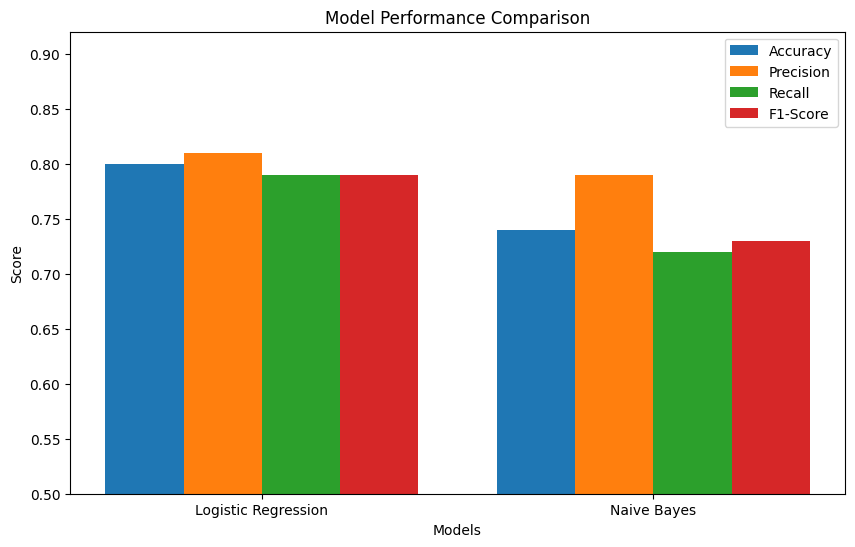
\includegraphics[width=0.75\linewidth]{model performance comparision.png}
    \caption{Model-Performance-Comparision}
    \label{fig:enter-label}
\end{figure}

\begin{table}[h]
    \centering
    \begin{tabular}{|l|c|c|c|c|}
        \hline
        \textbf{Model} & \textbf{Accuracy} & \textbf{Precision} & \textbf{Recall} & \textbf{F1-score} \\ \hline
        Logistic Regression & 80\% & 81\% & 79\% & 79\% \\ \hline
        Naïve Bayes & 74\% & 79\% & 72\% & 73\% \\ \hline
    \end{tabular}
    \caption{Performance Metrics Comparison of Different Models}
    \label{tab:model_comparison}
\end{table}

Key Observations:
    Logistic Regression (LR) achieved an accuracy of (80\%), with precision of (81\%) and recall of (79\%). This indicates that Logistic Regression was relatively good at identifying both positive and negative instances, although it was slightly more conservative in classifying certain products. With high precision and recall, it effectively balanced false positives and false negatives, which is critical for e-commerce tasks where correct product categorization is crucial.
    
    Naïve Bayes (NB), on the other hand, had a lower accuracy of (74\%), with precision of (79\%) and recall of (72\%). The lower recall suggests that Naïve Bayes struggled to correctly classify all the relevant products (positive instances), missing out on identifying some products accurately. This could mean that the model sometimes categorized relevant products incorrectly, which can be a challenge in e-commerce classification where missing important items could lead to poor customer experiences.
    
    
Takeaway:

Logistic Regression proves to be a strong and balanced model for classifying e-commerce product descriptions, offering a good compromise between precision and recall. Its ability to correctly identify relevant products while minimizing false positives makes it a reliable choice for product categorization tasks. 

\uline{Naive Bayes Analysis:}

\begin{figure}
    \centering
    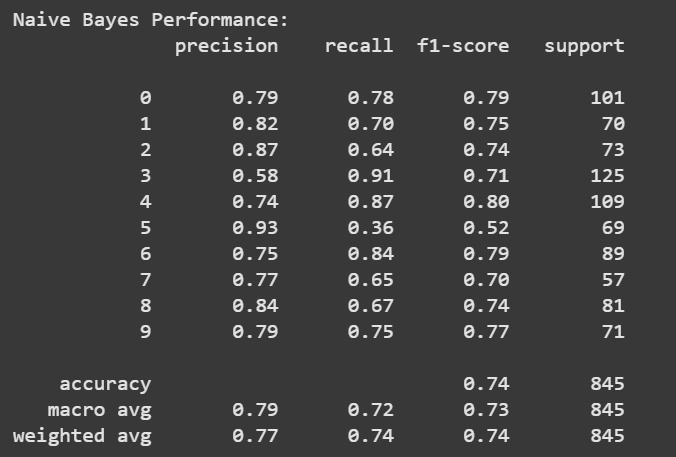
\includegraphics[width=0.75\linewidth]{naive bayes performance.png}
    \caption{Naive Bayes Performance}
    \label{fig:enter-label}
\end{figure}

Takeaway:

    Logistic Regression achieves balanced performance across all metrics, making it a reliable choice for general classification tasks.

    Naïve Bayes struggles with recall, which may lead to more false negatives in sensitive applications.

    Precision for Naïve Bayes is relatively high, making it suitable when false positives are more problematic than false negatives.



\uline{Attention Heatmap Analysis:}  

\begin{figure}
    \centering
    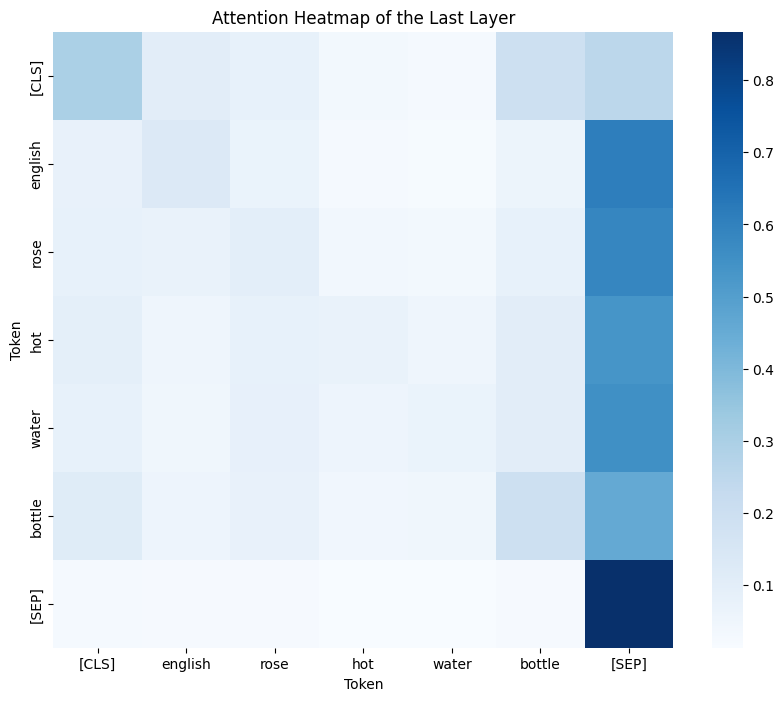
\includegraphics[width=0.75\linewidth]{attention heatmap.png}
    \caption{Attention-Heatmap}
    \label{fig:enter-label}
\end{figure}

   High Attention on Certain words
    Words like "english" and receive high attention, indicating that  country of origin play a role in classification.

    Focus on Specific Words
    Words like "bottle" and "water" receive moderate attention, suggesting a contextual link between these tokens.

    Limited Attention on Other Words
    Words like "rose" and "hot" have low attention values, indicating they contribute less to the model's final understanding.

    Potential Contextual Understanding
    The model appears to focus on specific tokens rather than uniformly distributing attention, implying it prioritizes certain word relationships over others.

\newpage



\section{5 Conclusion and Future Scope}

\subsection{5.1 Conclusion}


This project demonstrated the effectiveness of topic modeling techniques such as LDA and BERTopic in uncovering hidden structures within e-commerce product descriptions. By leveraging these methods, retailers can enhance product categorization, improve search relevance, and optimize recommendation systems. The integration of interactive dashboards further enables businesses to explore discovered topics dynamically, providing valuable market insights.

Future work can explore deep learning-based topic modeling approaches like neural LDA and transformer-based embeddings to capture more nuanced relationships within product descriptions. Additionally, integrating real-time topic tracking can help identify emerging trends in consumer preferences, allowing e-commerce platforms to adapt their strategies dynamically.

Another promising direction is the application of multilingual topic modeling to support global marketplaces, ensuring accurate categorization across different languages. Combining topic modeling with sentiment analysis could further refine product recommendations based on user sentiment trends. Overall, the project lays a strong foundation for AI-driven e-commerce enhancements, paving the way for more advanced, automated, and intelligent retail solutions.



\newpage
\subsection{5.2 Future Scope}

While this project achieved significant milestones, several potential areas for improvement and expansion exist:

\uline{Enhancing Model Performance:}

    Fine-tune larger transformer-based models such as RoBERTa, GPT, or T5 for improved accuracy.
    
    Use multi-modal approaches, integrating text, images, and metadata for more comprehensive analysis.

\uline{Improving Explainability \& Interpretability:}

    Extend SHAP and LIME analysis to multi-class problems for deeper insights into model decision-making.
    
    Explore causal inference techniques in NLP to better understand relationships between words and classifications.

\uline{Real-World Deployment \& Automation:}

    Deploy topic modeling results using Flask, FastAPI, or Streamlit to create interactive dashboards for exploring discovered product categories.

Integrate with e-commerce platforms to automatically categorize new products based on learned topic structures, enhancing search and recommendation systems.

\uline{Expanding to More Complex NLP Tasks:}

    Implement multi-task learning (MTL) where a single model performs multiple NLP tasks simultaneously 
    
    Investigate cross-lingual NLP models to extend the project’s impact to multiple languages.

\newpage

\section{References}

{[}1{]} Jacob Devlin, Ming-Wei Chang, Kenton Lee, and Kristina Toutanova. 2019. BERT: Pre-training of Deep Bidirectional Transformers for Language Understanding. In Proceedings of the 2019 Conference of the North American Chapter of the Association for Computational Linguistics: Human Language Technologies, Volume 1 (Long and Short Papers), pages 4171–4186, Minneapolis, Minnesota. Association for Computational Linguistics.

{[}2{]} Hannah Rashkin, Eunsol Choi, Jin Yea Jang, Svitlana Volkova, and Yejin Choi. 2017. Truth of Varying Shades: Analyzing Language in Fake News and Political Fact-Checking. In Proceedings of the 2017 Conference on Empirical Methods in Natural Language Processing, pages 2931–2937, Copenhagen, Denmark. Association for Computational Linguistics.

{[}3{]} Marco Tulio Ribeiro, Sameer Singh, and Carlos Guestrin. 2016. "Why Should I Trust You?": Explaining the Predictions of Any Classifier. In Proceedings of the 22nd ACM SIGKDD International Conference on Knowledge Discovery and Data Mining (KDD '16). Association for Computing Machinery, New York, NY, USA, 1135–1144. https://doi.org/10.1145/2939672.2939778

{[}4{]} https://huggingface.co/distilbert-base-uncased


\newpage
\begin{center}
    

\textbf{INDIVIDUAL CONTRIBUTION REPORT:}

\textbf{NLP  \&  TEXT-BASED MODELING}

SAHIL BINAKAR

22053712
\end{center}
\textbf{Abstract:} This project explores Natural Language Processing (NLP) techniques for text classification, sentiment analysis, and topic modeling. It involves building a pipeline for data preprocessing, implementing machine learning and transformer-based models (BERT, DistilBERT), and applying explainability techniques like LIME and SHAP. Datasets include Fake News Detection, Twitter US Airline Sentiment, and Amazon Reviews. Performance is evaluated using accuracy, F1-score, and confusion matrices. The project aims to enhance model interpretability and provide insights into textual data through advanced NLP methodologies.

\textbf{Individual contribution and findings:} During this project, my primary contribution was centered around Topic Modeling on E-Commerce Descriptions, focusing on data preprocessing, model development, performance evaluation, and analysis. I was responsible for building a structured NLP pipeline, implementing topic modeling techniques such as Latent Dirichlet Allocation (LDA) and Non-Negative Matrix Factorization (NMF), and conducting a comparative study to analyze their effectiveness in discovering hidden topics. Additionally, I worked on optimizing preprocessing steps, including tokenization, stopword removal, and lemmatization, to enhance topic coherence. To improve interpretability, I utilized word cloud visualizations and topic coherence scores to evaluate model performance and extract meaningful insights.

Findings \& Insights:

Logistic Regression outperformed Naïve Bayes across all metrics, achieving (80\%) accuracy with balanced precision (81\%) and recall (79\%).  

The topic distributions revealed that product descriptions often contain recurring themes related to material, usage, and seasonal trends, influencing model performance.  

Further analysis indicated that Naïve Bayes struggled with ambiguous terms, leading to lower recall (72\%) and reduced effectiveness in capturing less frequent but meaningful topics.



\textbf{Individual contribution to project report preparation:} I contributed significantly to the project report by writing Chapter 1 (Introduction) and Chapter 5 (Conclusion) while also structuring Chapter 2 (Basic Concepts/Literature Review),  Chapter 3 (Problem Statement) and Chapter 4 (Implementation) to ensure consistency across different datasets. Additionally, I took the lead in editing and refining the entire report, ensuring clarity, logical flow, and adherence to formatting standards. My efforts focused on making the document cohesive, technically accurate, and professionally structured for effective communication of our project’s objectives, methodologies, and findings.





\end{document}